\chapter{Filtro del PLL}
\section*{Resumen}

En este capítulo se presenta el diseño, desarrollo y caracterización del filtro activo utilizado en el PLL basado en el sintetizador ADF4159. El filtro fue diseñado para permitir la generación de una modulación FMCW con un barrido de $300~\mathrm{MHz}$ en un tiempo de $0{,}5~\mathrm{ms}$.

\section{Introducción}

El filtro constituye una de las etapas fundamentales de un PLL, debido a que determina la respuesta dinámica del sistema y permite generar la tensión de control aplicada al VCO a partir de los pulsos de corriente provenientes de la bomba de carga.

En una aplicación convencional de síntesis de frecuencia, el diseño del filtro suele orientarse a obtener un compromiso entre estabilidad, velocidad de respuesta, ruido de fase y rechazo de componentes espurias. Sin embargo, en el presente trabajo el PLL se utiliza para generar una señal FMCW mediante las funciones de modulación de rampa incorporadas en el ADF4159. Por este motivo, la capacidad de seguimiento de variaciones rápidas de frecuencia constituye el principal criterio de diseño.

El requerimiento establecido para el generador consiste en realizar barridos en forma de diente de sierra de $300~\mathrm{MHz}$ en $1~\mathrm{ms}$ y barridos triangulares de $300~\mathrm{MHz}$ por pendiente en un período de $0{,}5~\mathrm{ms}$; por lo tanto, el filtro debe proporcionar una dinámica suficientemente rápida para permitir el seguimiento de la rampa sin pérdida de enganche y manteniendo la linealidad.

\section{Parámetros de diseño}

Los principales parámetros considerados para el diseño del filtro se resumen en la Tabla~\ref{tab:parametros_filtro_lazo}.

\begin{table}[H]
\centering
\begin{tabular}{lc}
\hline
\textbf{Parámetro} & \textbf{Especificación} \\
\hline
Frecuencia de referencia del PFD & $50~\mathrm{MHz}$ \\
Frecuencia inicial & $1{,}55~\mathrm{GHz}$ \\
Frecuencia central & $1{,}70~\mathrm{GHz}$ \\
Frecuencia final & $1{,}85~\mathrm{GHz}$ \\
Ancho de banda del barrido & $300~\mathrm{MHz}$ \\
Tiempo de chirp diente de sierra & $1~\mathrm{ms}$ \\
Tiempo de chirp triangular & $0{,}5~\mathrm{ms}$ \\
Pendiente de frecuencia máxima & $1{,}2\times10^{12}~\mathrm{Hz/s}$ \\
Ancho de banda del PLL & $\approx290~\mathrm{kHz}$ \\
VCO & CVCO55BE-1530-2700 \\
Sintetizador & ADF4159 \\
\hline
\end{tabular}
\caption{Parámetros utilizados para el diseño del filtro.}
\label{tab:parametros_filtro_lazo}
\end{table}

La pendiente de frecuencia requerida para el barrido se obtiene como:

\begin{equation}
S_f = \frac{\Delta f}{T_{\mathrm{chirp}}} = \frac{300~\mathrm{MHz}}{0{,}25~\mathrm{ms}} = 1{,}2\times10^{12}~\mathrm{Hz/s}.
\end{equation}

Debido a la necesidad de seguir esta variación de frecuencia, se priorizó una respuesta dinámica rápida del PLL. Dado que en la literatura revisada no se encontró un criterio de diseño específicamente orientado a modulaciones FMCW con las características requeridas en este trabajo, se consultaron los recursos técnicos de Analog Devices. En particular, en \cite{AnalogDevices2015ADF4158} se presenta una metodología de diseño del filtro para los sintetizadores ADF4158 y ADF4159, basada en el uso de la herramienta \textit{ADIsimPLL}. Esta herramienta permite evaluar la respuesta del PLL y seleccionar los parámetros del filtro de acuerdo con los requerimientos de estabilidad y velocidad de respuesta para modulaciones de frecuencia, como se muestra en \cite{AnalogDevices2012ADIsimPLL}.

A partir de esta metodología se obtuvo, mediante \textit{ADIsimPLL}, un ancho de banda de lazo de aproximadamente $293~\mathrm{kHz}$ y un margen de fase de $48^\circ$. Estos valores fueron adoptados como referencia para el diseño y la configuración del sistema. Asimismo, se observó que la placa de evaluación del sintetizador ADF4159 emplea valores de ancho de banda y margen de fase de magnitud similar, lo que proporciona una referencia adicional para la selección de estos parámetros.

El siguiente paso del diseño consistió en verificar que el PLL fuera capaz de realizar el barrido completo del ancho de banda requerido. Para ello, fue necesario determinar el rango de tensión de control que debe aplicarse al VCO para cubrir las frecuencias comprendidas entre $1{,}55~\mathrm{GHz}$ y $1{,}85~\mathrm{GHz}$. Esta tensión constituye un parámetro fundamental para la selección de la topología del filtro, ya que debe garantizarse que la tensión de salida del filtro permanezca dentro del rango de operación del VCO durante todo el barrido.

En particular, la capacidad del filtro para convertir la corriente suministrada por la bomba de carga en la tensión de control requerida determina si una implementación pasiva resulta suficiente. Si el filtro pasivo no permite alcanzar el rango de tensión necesario para cubrir todo el intervalo de frecuencias, es necesario considerar una topología activa que proporcione la ganancia adicional requerida en la trayectoria de control.

El rango de tensión del VCO es:
\begin{equation}
\Delta V_{\text{tune}} = 3{,}15 - 1{,}19 = 1{,}96~\mathrm{V}.
\end{equation}

En \cite{adf4159}, la especificación de la bomba de carga establece que su tensión máxima de salida está limitada a $V_P - 0{,}5~\mathrm{V}$ (típicamente $2{,}8~\mathrm{V}$ para una alimentación de $3{,}3~\mathrm{V}$), un valor inferior a los $3{,}15~\mathrm{V}$ requeridos por el VCO; por lo tanto, para completar el rango de frecuencias se debe utilizar una topología activa.

Como explica \cite{harney_pll}, dentro de las topologías inversoras y no inversoras se destaca que la primera ofrece la ventaja de polarizar la salida de la bomba de carga a una tensión fija, típicamente la mitad de la tensión de la bomba de carga ($V_P/2$), lo cual resulta óptimo para el rendimiento frente a espurias. Además, es importante asegurarse de que el circuito integrado del PLL permita invertir la polaridad del PFD, lo cual es posible para el caso del ADF4159, por lo que se seleccionará la topología inversora.

Para obtener un buen desempeño se requiere un amplificador operacional con baja densidad de ruido de tensión para minimizar el ruido de fase, baja corriente de polarización de entrada para reducir las espurias y entradas \textit{rail-to-rail} cuando se utiliza una alimentación simple. El amplificador seleccionado y recomendado por \textit{ADIsimPLL} es el OP184 \cite{op184}, cuyas características más importantes para esta aplicación se exponen en la Tabla~\ref{tab:op184_specs}:

\begin{table}[H]
\centering
\begin{tabular}{lc}
\hline
\textbf{Parámetro} & \textbf{Especificación} \\
\hline
Tensión de alimentación & $3$--$36~\mathrm{V}$ \\
Rango de entrada & Rail-to-Rail \\
Rango de salida & Rail-to-Rail \\
Ancho de banda & $4~\mathrm{MHz}$ \\
Slew rate & $4{,}0~\mathrm{V}/\mu\mathrm{s}$ \\
Densidad de ruido de tensión & $3{,}9~\mathrm{nV}/\sqrt{\mathrm{Hz}}$ \\
\hline
\end{tabular}
\caption{Principales especificaciones del amplificador operacional OP184.}
\label{tab:op184_specs}
\end{table}

Para la selección del amplificador operacional se consideraron como criterios principales la velocidad de variación de la tensión de control, el rango de tensión de entrada y salida y la densidad de ruido. Para el barrido requerido, la tensión de sintonía debe variar desde $1{,}19~\mathrm{V}$ hasta $3{,}15~\mathrm{V}$ en un tiempo de $0{,}25~\mathrm{ms}$. Por lo tanto, el \textit{slew rate} mínimo requerido es $7{,}84~\mathrm{mV}/\mu\mathrm{s}$. El OP184 presenta un \textit{slew rate} de $4~\mathrm{V}/\mu\mathrm{s}$, entradas y salidas \textit{rail-to-rail}, y una densidad de ruido de tensión de $3{,}9~\mathrm{nV}/\sqrt{\mathrm{Hz}}$, inferior al valor de referencia de $10~\mathrm{nV}/\sqrt{\mathrm{Hz}}$. Por lo tanto, el dispositivo cumple los requerimientos de velocidad y rango de tensión, mientras que su bajo ruido permite minimizar la contribución del filtro activo al ruido de fase del PLL.

Para el diseño del filtro se tomó como referencia la metodología recomendada por Analog Devices, fabricante del PLL utilizado, específicamente las consideraciones presentadas para los dispositivos ADF4158 y ADF4159 en \cite{AnalogDevices2015ADF4158}. Asimismo, para la selección y ajuste de los componentes del filtro se siguió el procedimiento de diseño y simulación mediante la herramienta \textit{ADIsimPLL}, recomendada por Analog Devices para el análisis del comportamiento del PLL y, en particular, para la simulación de barridos de frecuencia, tal como se presenta en \cite{AnalogDevices2012ADIsimPLL}. De esta manera, los parámetros del filtro se determinaron siguiendo la metodología propuesta por el propio fabricante, adaptándola a los requerimientos específicos de ancho de banda, estabilidad y rango de tensión de control del sistema diseñado.

Como se desarrolló en la Subsección~\ref{subsec:filtrolazomarco}, los polos y ceros de la función de transferencia son los siguientes:

\begin{itemize}
\item Polo de la bomba de carga:
\begin{equation}
\omega_{p4} = \frac{1}{R_1 C_1}.
\end{equation}

\item Cero:
\begin{equation}
\omega_z = \frac{1}{R_2 C_2}.
\end{equation}

\item Polo en el origen:
\begin{equation}
\omega_{p1} = 0.
\end{equation}

\item Segundo polo:
\begin{equation}
\omega_{p2} = \frac{C_2 + C_3}{R_2 C_2 C_3}.
\end{equation}

\item Polo de salida:
\begin{equation}
\omega_{p3} = \frac{1}{R_3 (C_4 + C_{\mathrm{VCO}})}.
\end{equation}
\end{itemize}

Los componentes pasivos seleccionados en \textit{ADIsimPLL} son los siguientes:
\begin{itemize}
  \item $C_1 = 220~\mathrm{pF}$
  \item $R_1 = 100~\Omega$
  \item $R_2 = 180~\Omega$
  \item $C_2 = 8{,}2~\mathrm{nF}$
  \item $C_3 = 220~\mathrm{pF}$
  \item $R_3 = 820~\Omega$
  \item $C_4 = 180~\mathrm{pF}$
  \item $C_{\mathrm{VCO}} = 50{,}0~\mathrm{pF}$
\end{itemize}

Los polos y ceros mencionados anteriormente quedan:
\begin{itemize}
  \item Polo en el origen:
  \begin{equation}
    \omega_{p1} = 0~\mathrm{rad/s}
  \end{equation}

  \item Cero:
  \begin{equation}
    \omega_z = 6{,}77 \times 10^5~\mathrm{rad/s} \quad (107{,}8~\mathrm{kHz})
  \end{equation}

  \item Segundo polo:
  \begin{equation}
    \omega_{p2} = 2{,}59 \times 10^7~\mathrm{rad/s} \quad (4{,}13~\mathrm{MHz})
  \end{equation}

  \item Polo de salida:
  \begin{equation}
    \omega_{p3} = 5{,}30 \times 10^6~\mathrm{rad/s} \quad (843{,}6~\mathrm{kHz})
  \end{equation}

  \item Polo de la bomba de carga:
  \begin{equation}
    \omega_{p4} = 4{,}54 \times 10^7~\mathrm{rad/s} \quad (7{,}23~\mathrm{MHz})
  \end{equation}
\end{itemize}

En la Figura~\ref{fig:componentes} se muestran los componentes del filtro.

\begin{figure}[H]
    \centering
    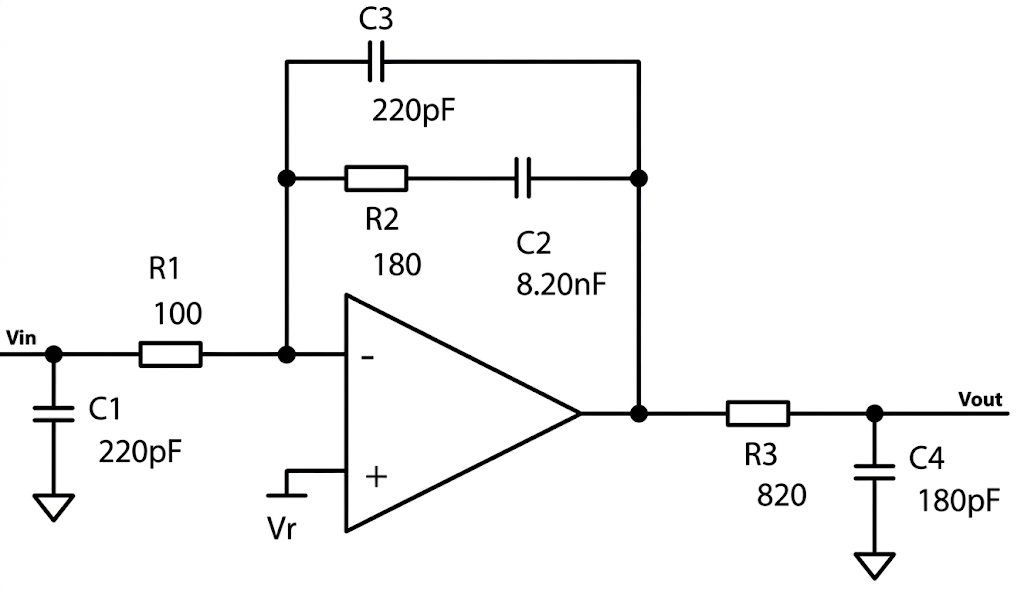
\includegraphics[width=0.75\linewidth]{imagenes/componentesfiltrolazo.png}
    \caption{Componentes del filtro. (Fuente: propia).}
    \label{fig:componentes}
\end{figure}

Desde el punto de vista de la estabilidad, la estructura seleccionada para el filtro resulta adecuada para los requerimientos del sistema completo, ya que permite obtener un error de fase estacionario nulo frente a una entrada de tipo rampa, condición necesaria para reproducir adecuadamente el barrido de frecuencia requerido por el radar FMCW.

Por otra parte, el cero ubicado aproximadamente en $107{,}8~\mathrm{kHz}$ cumple un papel fundamental en la estabilidad del lazo. De esta manera, se incrementa el margen de fase del sistema y se evita que la frecuencia de cruce se encuentre próxima a una condición de inestabilidad.

Finalmente, los polos adicionales del filtro, ubicados en un rango aproximado de $800~\mathrm{kHz}$ a $7{,}2~\mathrm{MHz}$, se encuentran suficientemente alejados de la frecuencia de cruce del lazo. Esto permite atenuar las componentes de alta frecuencia provenientes del detector de fase y de la bomba de carga, reduciendo el ruido que puede alcanzar al VCO, sin afectar significativamente el margen de fase establecido por el cero principal.

Con el objetivo de verificar el comportamiento del filtro antes de su implementación, se realizó una simulación teórica utilizando MATLAB. En esta etapa se evaluó la respuesta del filtro a partir de los valores de los componentes obtenidos mediante la metodología de diseño presentada anteriormente. La simulación permite analizar la respuesta en frecuencia del filtro y comprobar que su comportamiento resulta compatible con los requerimientos establecidos para el sistema PLL. En la Figura~\ref{fig:filtrolazomatl} se presentan los resultados obtenidos mediante MATLAB.

\begin{figure}[H]
    \centering
    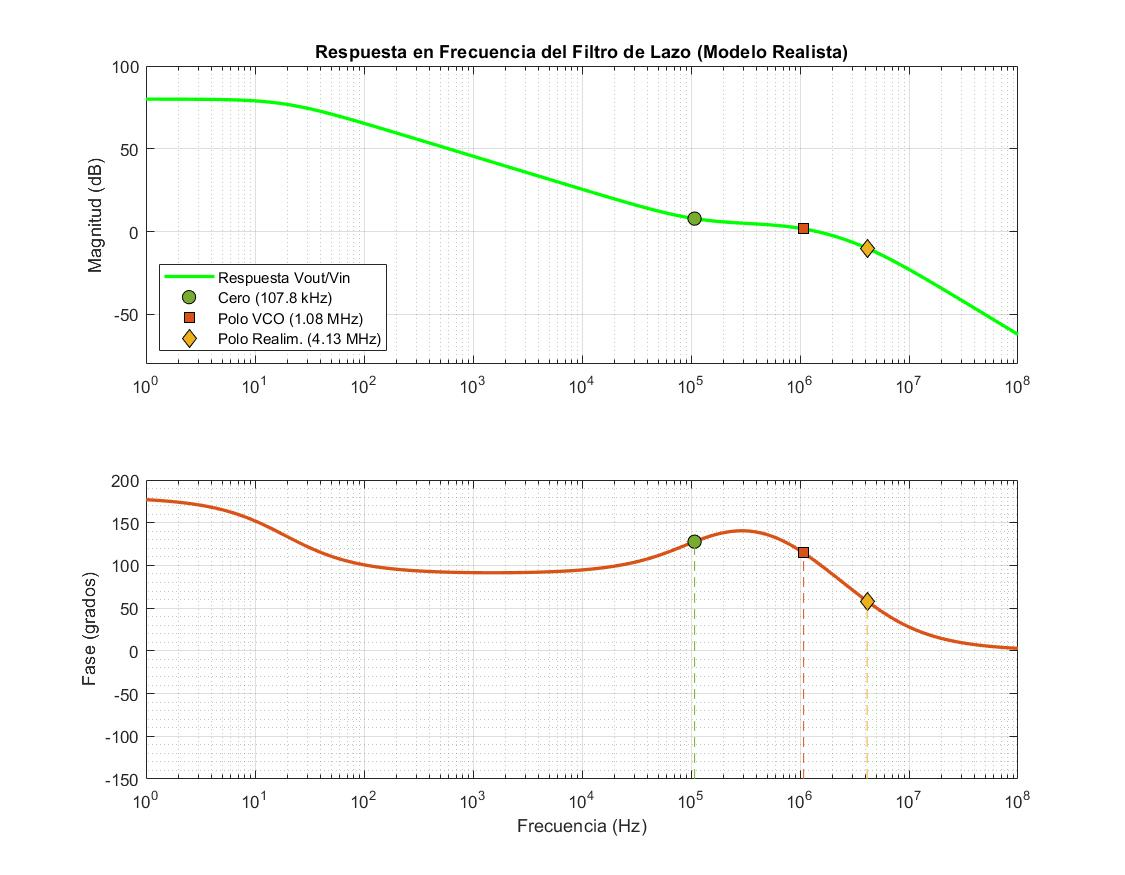
\includegraphics[width=0.75\linewidth]{imagenes/filtrolazorta.jpg}
    \caption{Respuesta teórica del filtro. (Fuente: propia).}
    \label{fig:filtrolazomatl}
\end{figure}

\section{Simulación}
Con el objetivo de verificar el comportamiento del filtro antes de su integración en el PLL, se realizó una simulación a nivel circuital utilizando Multisim. Para ello, se implementó el circuito correspondiente a la topología seleccionada utilizando los valores de los componentes obtenidos mediante el procedimiento de diseño basado en \textit{ADIsimPLL}. Esta simulación permite verificar el comportamiento eléctrico del filtro y comprobar que los valores seleccionados producen una respuesta consistente con el análisis teórico realizado previamente.

En la Figura~\ref{fig:filtrolazsim} se presenta el circuito implementado. Los resultados permiten observar el comportamiento del filtro frente a las variaciones de la señal de entrada y verificar la generación de la tensión de control requerida para el VCO. De esta manera, la simulación constituye una primera validación del diseño a nivel circuital, previo a su incorporación al modelo completo del PLL.

\begin{figure}[H]
    \centering
    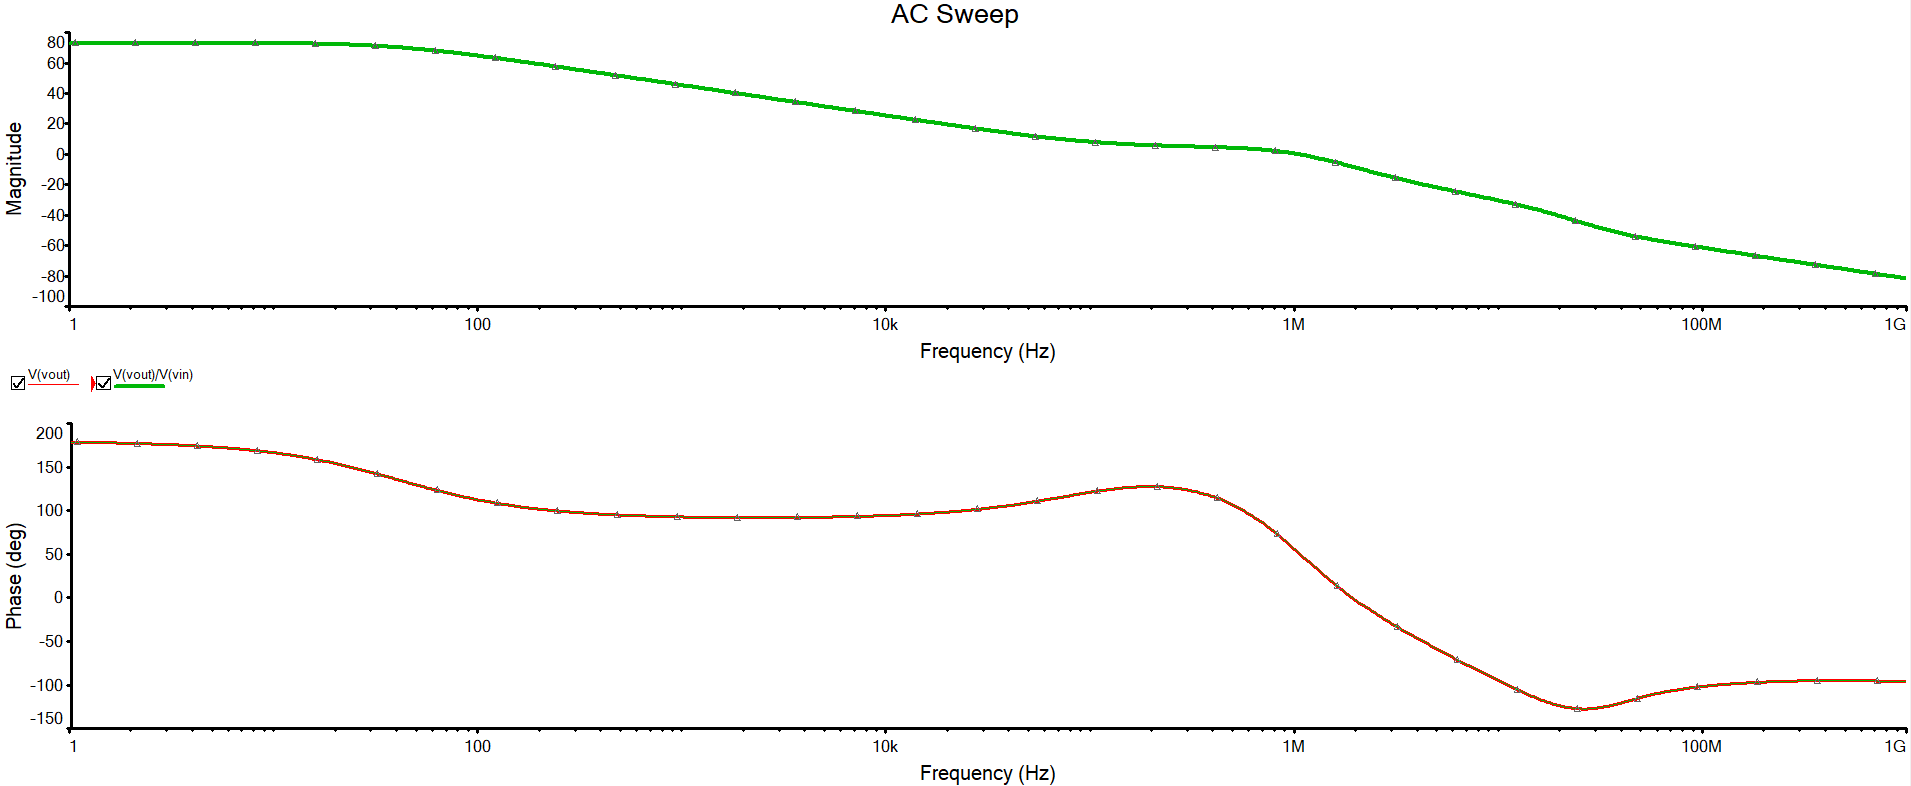
\includegraphics[width=0.75\linewidth]{imagenes/filtrolazsim.png}
    \caption{Simulación del filtro en Multisim. (Fuente: propia).}
    \label{fig:filtrolazsim}
\end{figure}

El análisis del comportamiento del filtro dentro del lazo completo se realizará posteriormente en la sección correspondiente al PLL. En dicha etapa se incorporarán el detector de fase y frecuencia, la bomba de carga, el divisor de frecuencia y el VCO, permitiendo analizar la respuesta dinámica del sistema completo y su capacidad para realizar el barrido de frecuencia requerido para la aplicación FMCW.

\section{Construcción del bloque}

Una vez finalizado el diseño y verificado el comportamiento del filtro mediante las simulaciones presentadas en la sección anterior, se procedió a la construcción del bloque correspondiente al filtro del PLL. El diseño de la placa de circuito impreso (PCB) se realizó utilizando el software \textit{KiCad}, a partir del esquemático eléctrico definido previamente.

Para la implementación se seleccionaron componentes comerciales disponibles en el mercado, procurando mantener los valores obtenidos durante el diseño del filtro y utilizar encapsulados adecuados para el montaje sobre PCB. Los componentes utilizados corresponden a las resistencias y capacitores que conforman la red de filtrado, junto con el amplificador operacional OP184 utilizado en la implementación de la topología activa.

La selección de los componentes se realizó considerando no solamente su valor nominal, sino también su disponibilidad, encapsulado y características eléctricas. Los capacitores utilizados corresponden a componentes cerámicos multicapa, mientras que las resistencias son componentes de montaje superficial. Los valores seleccionados se resumen a continuación:

\begin{table}[H]
\centering
\begin{tabular}{ccc}
\hline
\textbf{Componente} & \textbf{Valor nominal} & \textbf{Fabricante / modelo} \\
\hline
$C_1$ & $220~\mathrm{pF}$ & Murata GRT0335C1H221FA02D \\
$R_1$ & $100~\Omega$ & Yageo RT1206DRE07100RL \\
$R_2$ & $180~\Omega$ & Stackpole RMCF1206FT180R \\
$C_2$ & $8{,}2~\mathrm{nF}$ & Cal-Chip GMC21CG822F50NT \\
$C_3$ & $220~\mathrm{pF}$ & Murata GRT0335C1H221FA02D \\
$R_3$ & $820~\Omega$ & Yageo RT1206FRE07820RL \\
$C_4$ & $180~\mathrm{pF}$ & Murata GCM1555C1H181FA16D \\
\hline
\end{tabular}
\caption{Componentes utilizados en la implementación del filtro del PLL.}
\label{tab:componentes_filtro}
\end{table}

Además de los componentes que conforman la red de filtrado, se incorporó el amplificador operacional OP184, seleccionado durante la etapa de diseño debido a sus características de ruido, velocidad y rango de operación. Este dispositivo constituye el elemento activo de la topología seleccionada y permite obtener el rango de tensión de control requerido por el VCO.

Para facilitar la conexión del bloque con el resto del sistema se incorporaron dos conectores SMA. Uno de ellos corresponde a la entrada del bloque, utilizada para recibir la señal proveniente de la bomba de carga, mientras que el segundo corresponde a la salida del filtro, donde se obtiene la tensión de control destinada al VCO. La utilización de conectores SMA permite realizar conexiones mediante cable coaxial y facilita tanto la integración del bloque con el resto del sistema como la realización de mediciones durante la etapa experimental.

Adicionalmente, se incorporó un capacitor de desacople de $0{,}1~\mu\mathrm{F}$ asociado al terminal no inversor del amplificador operacional y al terminal de alimentación. Este componente forma parte de la red utilizada para establecer y estabilizar la referencia aplicada a dicha entrada, contribuyendo a reducir las variaciones de alta frecuencia que podrían introducir perturbaciones en la tensión de control del VCO.

El diseño de la PCB se realizó en \textit{KiCad}, trasladando el esquemático previamente definido al diseño físico de la placa. En la Figura~\ref{fig:pcb_filtro} se presenta la placa de circuito impreso fabricada, a la cual se le aplicó una capa de máscara UV para un mejor acabado y protección.

La disposición física de los componentes se realizó procurando mantener agrupados los elementos pertenecientes a la red de filtrado y ubicar el amplificador operacional próximo a dichos componentes. Los conectores SMA se colocaron en los extremos de la placa para facilitar la conexión con el resto del sistema y permitir el acceso a los puntos de entrada y salida del bloque.

\begin{figure}[H]
\centering
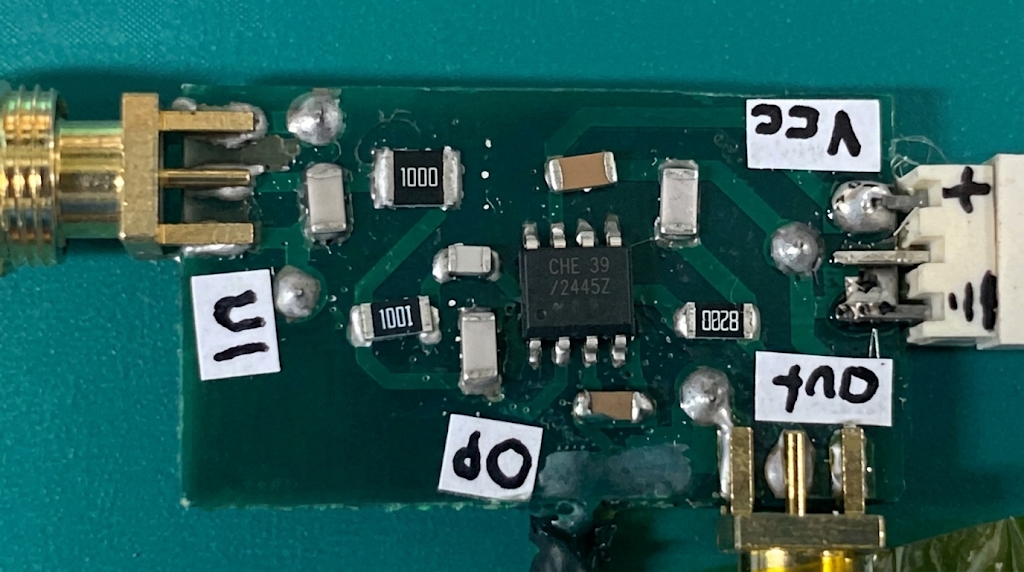
\includegraphics[width=0.75\linewidth]{imagenes/pcb_filtro.png}
\caption{Placa de circuito impreso del filtro del PLL desarrollado. (Fuente: propia).}
\label{fig:pcb_filtro}
\end{figure}

\subsection{Medición}

Los resultados obtenidos mediante la medición se presentan en la Figura~\ref{fig:frecmedidafiltro}, cuyos datos fueron graficados en MATLAB. La frecuencia de corte medida no coincide de forma directa con el ancho de banda del lazo calculado debido a que este último engloba la dinámica de todo el lazo del PLL (incluyendo el detector, la bomba de carga y el VCO) y no únicamente al filtro activo aislado. Aun así, el comportamiento medido exhibe una adecuada correlación con respecto al análisis teórico y a las simulaciones. Cabe destacar que la medición a lazo cerrado resulta compleja de aislar en frecuencia pura, por lo que se empleará el tiempo de respuesta y la linealidad temporal de la rampa para su verificación completa; adicionalmente, en frecuencias muy bajas el amplificador operacional tiende a saturar en mediciones directas a lazo abierto.

\begin{figure}[H]
\centering
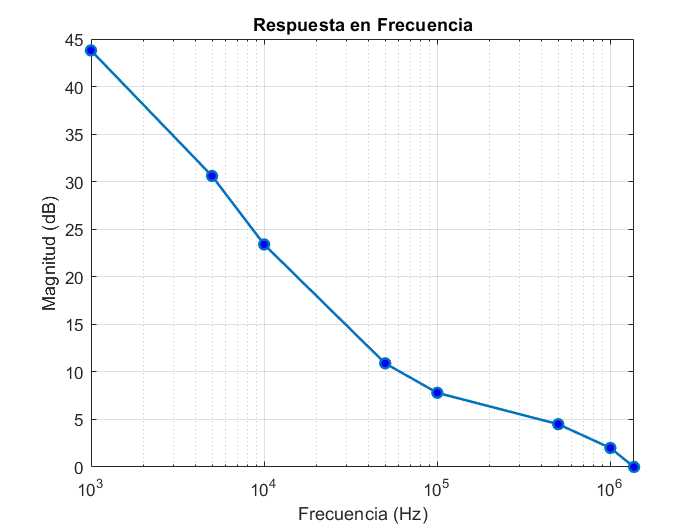
\includegraphics[width=0.5\linewidth]{imagenes/frecmedidafiltro.png}
\caption{Medición de la respuesta del filtro fabricado. (Fuente: propia).}
\label{fig:frecmedidafiltro}
\end{figure}

En particular, el cero calculado se encuentra alrededor de los $110~\mathrm{kHz}$, mientras que el primer polo de la red se ubica aproximadamente en $1.2~\mathrm{MHz}$.